\documentclass[../main/Notes.tex]{subfiles}
\begin{document}

\section[Solution 9: Everyday Predictions]{Solution 9: Everyday Predictions \iftoggle{showdates}{\small{\textit{2014-07-18}}}{}}

\subsection*{Exercise 1}
First we plot the prior distribution for some $\beta$ to get a feeling for it.
\begin{figure}[h]
  \centering
  \begin{tikzpicture}
    \begin{axis}[every axis plot post/.append style={mark=none, samples=50, smooth}, 
                  axis x line*=bottom, axis y line*=left, enlargelimits=upper, domain=0:10]
      \addplot[red]    {specErlang(0.25)};
        \addlegendentry{$\beta=0.25$}
      \addplot[green]  {specErlang(0.5)};
        \addlegendentry{$\beta=0.5$}
      \addplot[blue]   {specErlang(1)};
        \addlegendentry{$\beta=1$}
      \addplot[yellow] {specErlang(2)};
        \addlegendentry{$\beta=2$}
      \addplot[violet] {specErlang(3)};
        \addlegendentry{$\beta=3$}
    \end{axis}
  \end{tikzpicture}
  \caption{Special case of the Erlang distribution $\beta^{-2}xe^{-\frac{x}{\beta}}$ with different $\beta$.}
\end{figure}
We can easily see that a smaller $\beta$ causes a very high peak, while bigger $\beta$ caus the peak to flatten and move to the right.

\bigskip

After we got a feeling for the prior distribution, let's calculate the posterior distribution to make a guess, how long the total term of the member of the House of Representatives will be.

Let $X$ be the total time and $Y$ the observed value, i.e. the time we heard.

Then we can use Bayes' rule\index{Bayes' Rule} to come up with a solution. We use the distribution from the sheet for $p(Y=y|X=x) = \frac{1}{x}\mathcal{I}(y \leq x)$ as the likelihood and also plug in the given prior distribution $\beta^{-2}x e^{-\frac{x}{\beta}}$. Note that $\mathcal{I}(y \leq x)$ is the indication function, i.e. it is 1 if $y \leq x$ and 0 otherwise.

\begin{align*}
p(X=x|Y=y) &= \frac{p(Y=y|X=x)p(X=x)}{p(Y=y)} \\
           &= \frac{\frac{1}{x} \mathcal{I}(y \leq x) \beta^{-2} x e^{-\frac{x}{\beta}}}{p(Y=y)} \\
           &= \frac{\mathcal{I}(y \leq x) \beta^{-2} e^{-\frac{x}{\beta}}}{p(Y=y)}
\end{align*}
We can derive $p(Y=y)$ (normalization) by taking the integral of $e^{-\frac{x}{\beta}}\mathcal{I}(y \leq x)$.

\begin{align*}
p(Y=y) &= \int\limits_0^\infty e^{-\frac{x}{\beta}} \mathcal{I}(y \leq x) dx \\
       &= \int\limits_y^\infty e^{-\frac{x}{\beta}} dx = \left[-\beta e^{-\frac{x}{\beta}} \right]_y^\infty \\
       &= -\beta \cdot 0 + \beta e^{-\frac{y}{\beta}}
\end{align*}

By employing $p(Y=y)$ in the formula, we finally come up with our posterior distribution:
\begin{align*}
p(X=x|Y=y) &= \frac{\mathcal{I}(y \leq x) \beta^{-2} e^{-\frac{x}{\beta}}}{p(Y=y)} \\
           &= \frac{\mathcal{I}(y \leq x) \beta^{-2} e^{-\frac{x}{\beta}}}{\beta e^{-\frac{y}{\beta}}} \\
           &= \mathcal{I}(y \leq x) \frac{\beta^{-2} e^{-\frac{x}{\beta}}}{\beta e^{-\frac{y}{\beta}}}
\end{align*}

The plot of the posterior distribution is as follows (for a $y = 2$ and $\beta$ from $\left\{0.25, 0.5, 1, 2\right\}$).
\begin{figure}[h]
  \centering
  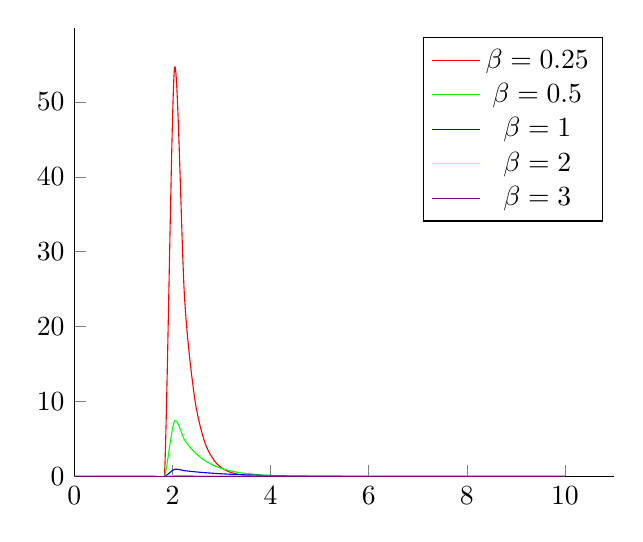
\begin{tikzpicture}
    \begin{axis}[every axis plot post/.append style={mark=none, samples=50, smooth}, 
                  axis x line*=bottom, axis y line*=left, enlargelimits=upper, domain=0:10]
      \addplot[red] {(2<=x) * ( 0.25^(-2) * exp(-x/0.25) ) / ( 0.25 * exp(-2/0.25) ) };
        \addlegendentry{$\beta=0.25$}
      \addplot[green] {(2<=x) * ( 0.5^(-2) * exp(-x/0.5) ) / ( 0.5 * exp(-2/0.5) ) };
        \addlegendentry{$\beta=0.5$}
      \addplot[blue] {(2<=x) * ( 1^(-2) * exp(-x/1) ) / ( 1 * exp(-2/1) ) };
        \addlegendentry{$\beta=1$}
      \addplot[yellow] {(2<=x) * ( 2^(-2) * exp(-x/2) ) / ( 2 * exp(-2/2) ) };
        \addlegendentry{$\beta=2$}
      \addplot[violet] {(2<=x) * ( 3^(-2) * exp(-x/3) ) / ( 3 * exp(-2/3) ) };
        \addlegendentry{$\beta=3$}
    \end{axis}
  \end{tikzpicture}
  \caption{Final posterior distribution.}
\end{figure}


\subsection*{Exercises 2 and 3}
\emph{Maybe added later...}

\end{document}